\documentclass[12pt]{article}

\usepackage{parskip}
\usepackage{listings}
\usepackage[charter]{mathdesign}
\usepackage{nimbusmono}
\usepackage{hyperref}
\usepackage[margin=1in]{geometry}
\usepackage{graphicx}

\lstset{
    language=C,
    basicstyle=\small\ttfamily,
    xleftmargin=1em
}

\author{Jesse op den Brouw\thanks{Please mail me at: \href{mailto:J.E.J.opdenBrouw@hhs.nl}{J.E.J.opdenBrouw@hhs.nl}}\\The Hague University of Applied Sciences\\(THUAS)}
\title{Graphic LCD and Touchscreen Functions for Velleman VMA412 with ILI9341 Controller used with a STM32F446 Nucleo Board}
\date{\today}


\begin{document}
\raggedbottom
\maketitle

\vfill
{\small\leftskip=1em\rightskip=1em
The Velleman VM412 is an Arduino Uno/Mega compatible 2.8" color Graphic LCD with 320x240 pixels controlled by an ILI9431 graphic controller. The ILI9431 is connected using an 8-bit 8080 interface to the board. More information can be found via \url{https://www.velleman.eu/products/view/?id=435582}. There are a number second sources for this board such as the Makerfactory 2.8" Touchscreen and the ELEGOO UNO R3 2.8 Inches TFT Touch Screen.

The software is written in C and consists of four driver files and one C test file.

Functions include plotting a pixel, rectangles, circles, arcs, printing strings and filling an object, and reading X, Y and pressure values. It also has primitive console based printing functions.

The software uses 18-bit colors where each color has 6 bits used.

The software is tested using a STM32F446 Nucleo board and STMCubeIDE version 1.3.1.

The VMA412 has a SD-card socket. This software has \textbf{no} support for accessing SD-cards.

}
\vfill

\newpage
\tableofcontents


\newpage

\section{Software License}
This software is licensed with the BSD License:

\begin{lstlisting}[basicstyle=\footnotesize\ttfamily]
Software License Agreement (BSD License)

Copyright (c) 2020 Jesse op den Brouw.  All rights reserved.

Portions based on :
 Copyright (c) 2012 Adafruit Industries.  All rights reserved.

Redistribution and use in source and binary forms, with or without
modification, are permitted provided that the following conditions are met:

- Redistributions of source code must retain the above copyright notice,
  this list of conditions and the following disclaimer.
- Redistributions in binary form must reproduce the above copyright notice,
  this list of conditions and the following disclaimer in the documentation
  and/or other materials provided with the distribution.

THIS SOFTWARE IS PROVIDED BY THE COPYRIGHT HOLDERS AND CONTRIBUTORS "AS IS"
AND ANY EXPRESS OR IMPLIED WARRANTIES, INCLUDING, BUT NOT LIMITED TO, THE
IMPLIED WARRANTIES OF MERCHANTABILITY AND FITNESS FOR A PARTICULAR PURPOSE
ARE DISCLAIMED. IN NO EVENT SHALL THE COPYRIGHT HOLDER OR CONTRIBUTORS BE
LIABLE FOR ANY DIRECT, INDIRECT, INCIDENTAL, SPECIAL, EXEMPLARY, OR
CONSEQUENTIAL DAMAGES (INCLUDING, BUT NOT LIMITED TO, PROCUREMENT OF
SUBSTITUTE GOODS OR SERVICES; LOSS OF USE, DATA, OR PROFITS; OR BUSINESS
INTERRUPTION) HOWEVER CAUSED AND ON ANY THEORY OF LIABILITY, WHETHER IN
CONTRACT, STRICT LIABILITY, OR TORT (INCLUDING NEGLIGENCE OR OTHERWISE)
ARISING IN ANY WAY OUT OF THE USE OF THIS SOFTWARE, EVEN IF ADVISED OF THE
POSSIBILITY OF SUCH DAMAGE.
\end{lstlisting}


\section{Documentation License}
This documentation is licensed with the Latex Project Public License:

\begin{lstlisting}[basicstyle=\footnotesize\ttfamily,showspaces=false]
Copyright 20205 J.E.J. op den BRouw

This work may be distributed and/or modified under the
conditions of the LaTeX Project Public License, either version 1.3
of this license or (at your option) any later version.
The latest version of this license is in
  http://www.latex-project.org/lppl.txt
and version 1.3 or later is part of all distributions of LaTeX
version 2005/12/01 or later.

This work has the LPPL maintenance status `maintained'.
 
The Current Maintainer of this work is J.E.J. op den Brouw.
\end{lstlisting}


\section{Mouting the VMA412}
The Velleman VM412 is an Arduino Uno/Mega compatible 2.8" color Graphic LCD with 320x240 pixels controlled by an ILI9431 graphic controller.
The VMA412 has an Arduino Uno compatible connection and can be connected to numerous STM32F Nucleo boards.
Place the VM412 board as instructed. See Figure~\ref{fig:1} for a visual inspection.

\begin{figure}[!ht]
\centering
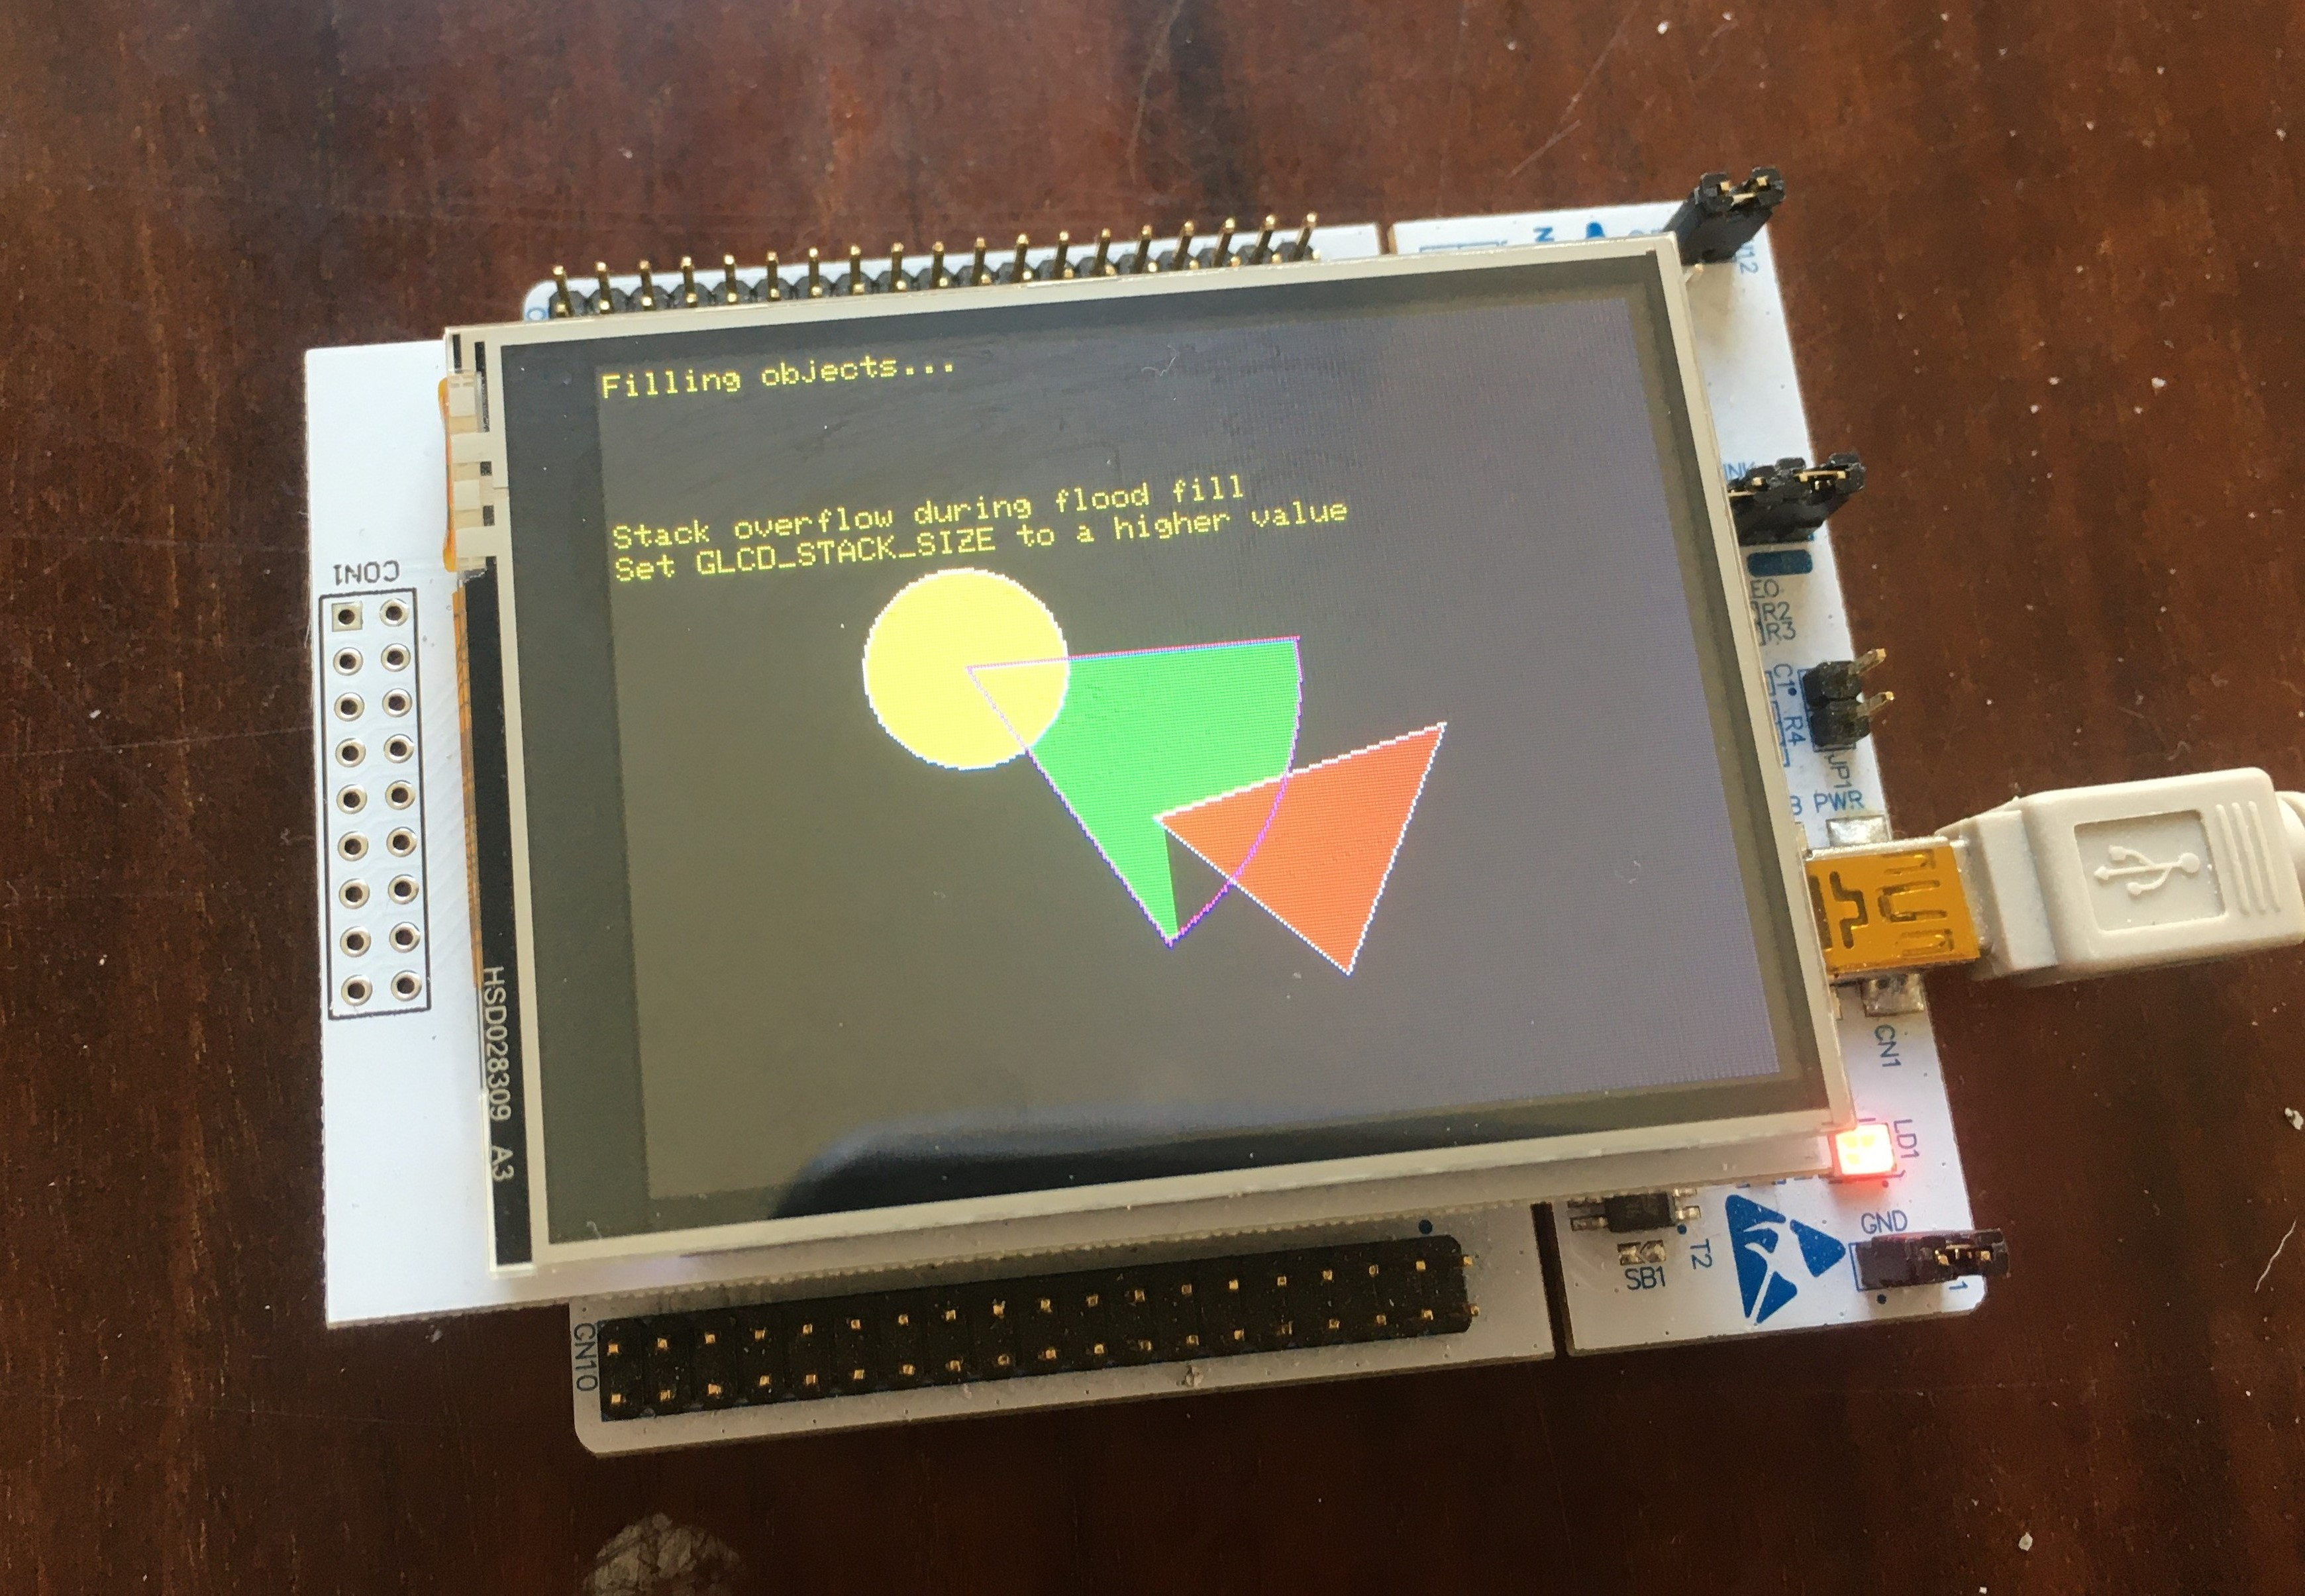
\includegraphics[width=0.7\textwidth]{glcd_demo}
\caption{Showing the VMA412 mounted on a STM32F446 Nucleo board.}
\label{fig:1}
\end{figure}



\section{Creating a project}
With STM32CubeIde, create a standard project for a STM32F446RE microcontroller. There is no need to
create a board project, just a chip project. 

After creating a project, just place the five files in the appropriate folders. There are five files:

\begin{lstlisting}
glcd_ili9341_vma412.h   -- place in Core/Inc, definitions, typedefs etc
glcd_ili9341_vma412.c   -- place in Core/Src, functions to call
touchscreen_vma412.h    -- place in Core/Inc, definitions, typedefs etc
touchscreen_vma412.c    -- place in Core/Src, functions to call
main.c                  -- place in Core/Src, demo using functions
\end{lstlisting}

\section{Running the demo}
Place the files in the appropriate folders and start compilation using \texttt{Project}$\rightarrow$\texttt{Build Project}.
Then start the the demo using \texttt{Run}$\rightarrow$\texttt{Run}. The demo starts by asking you to touch one of two rectangles to start the GLCD demo or the touchscreen demo, see Figure~\ref{fig:2}. At the end of the GLCD demo, there will be a list of running times for selected graphic functions as can be seen in Figure~\ref{fig:3}.

\begin{figure}[!ht]
\centering
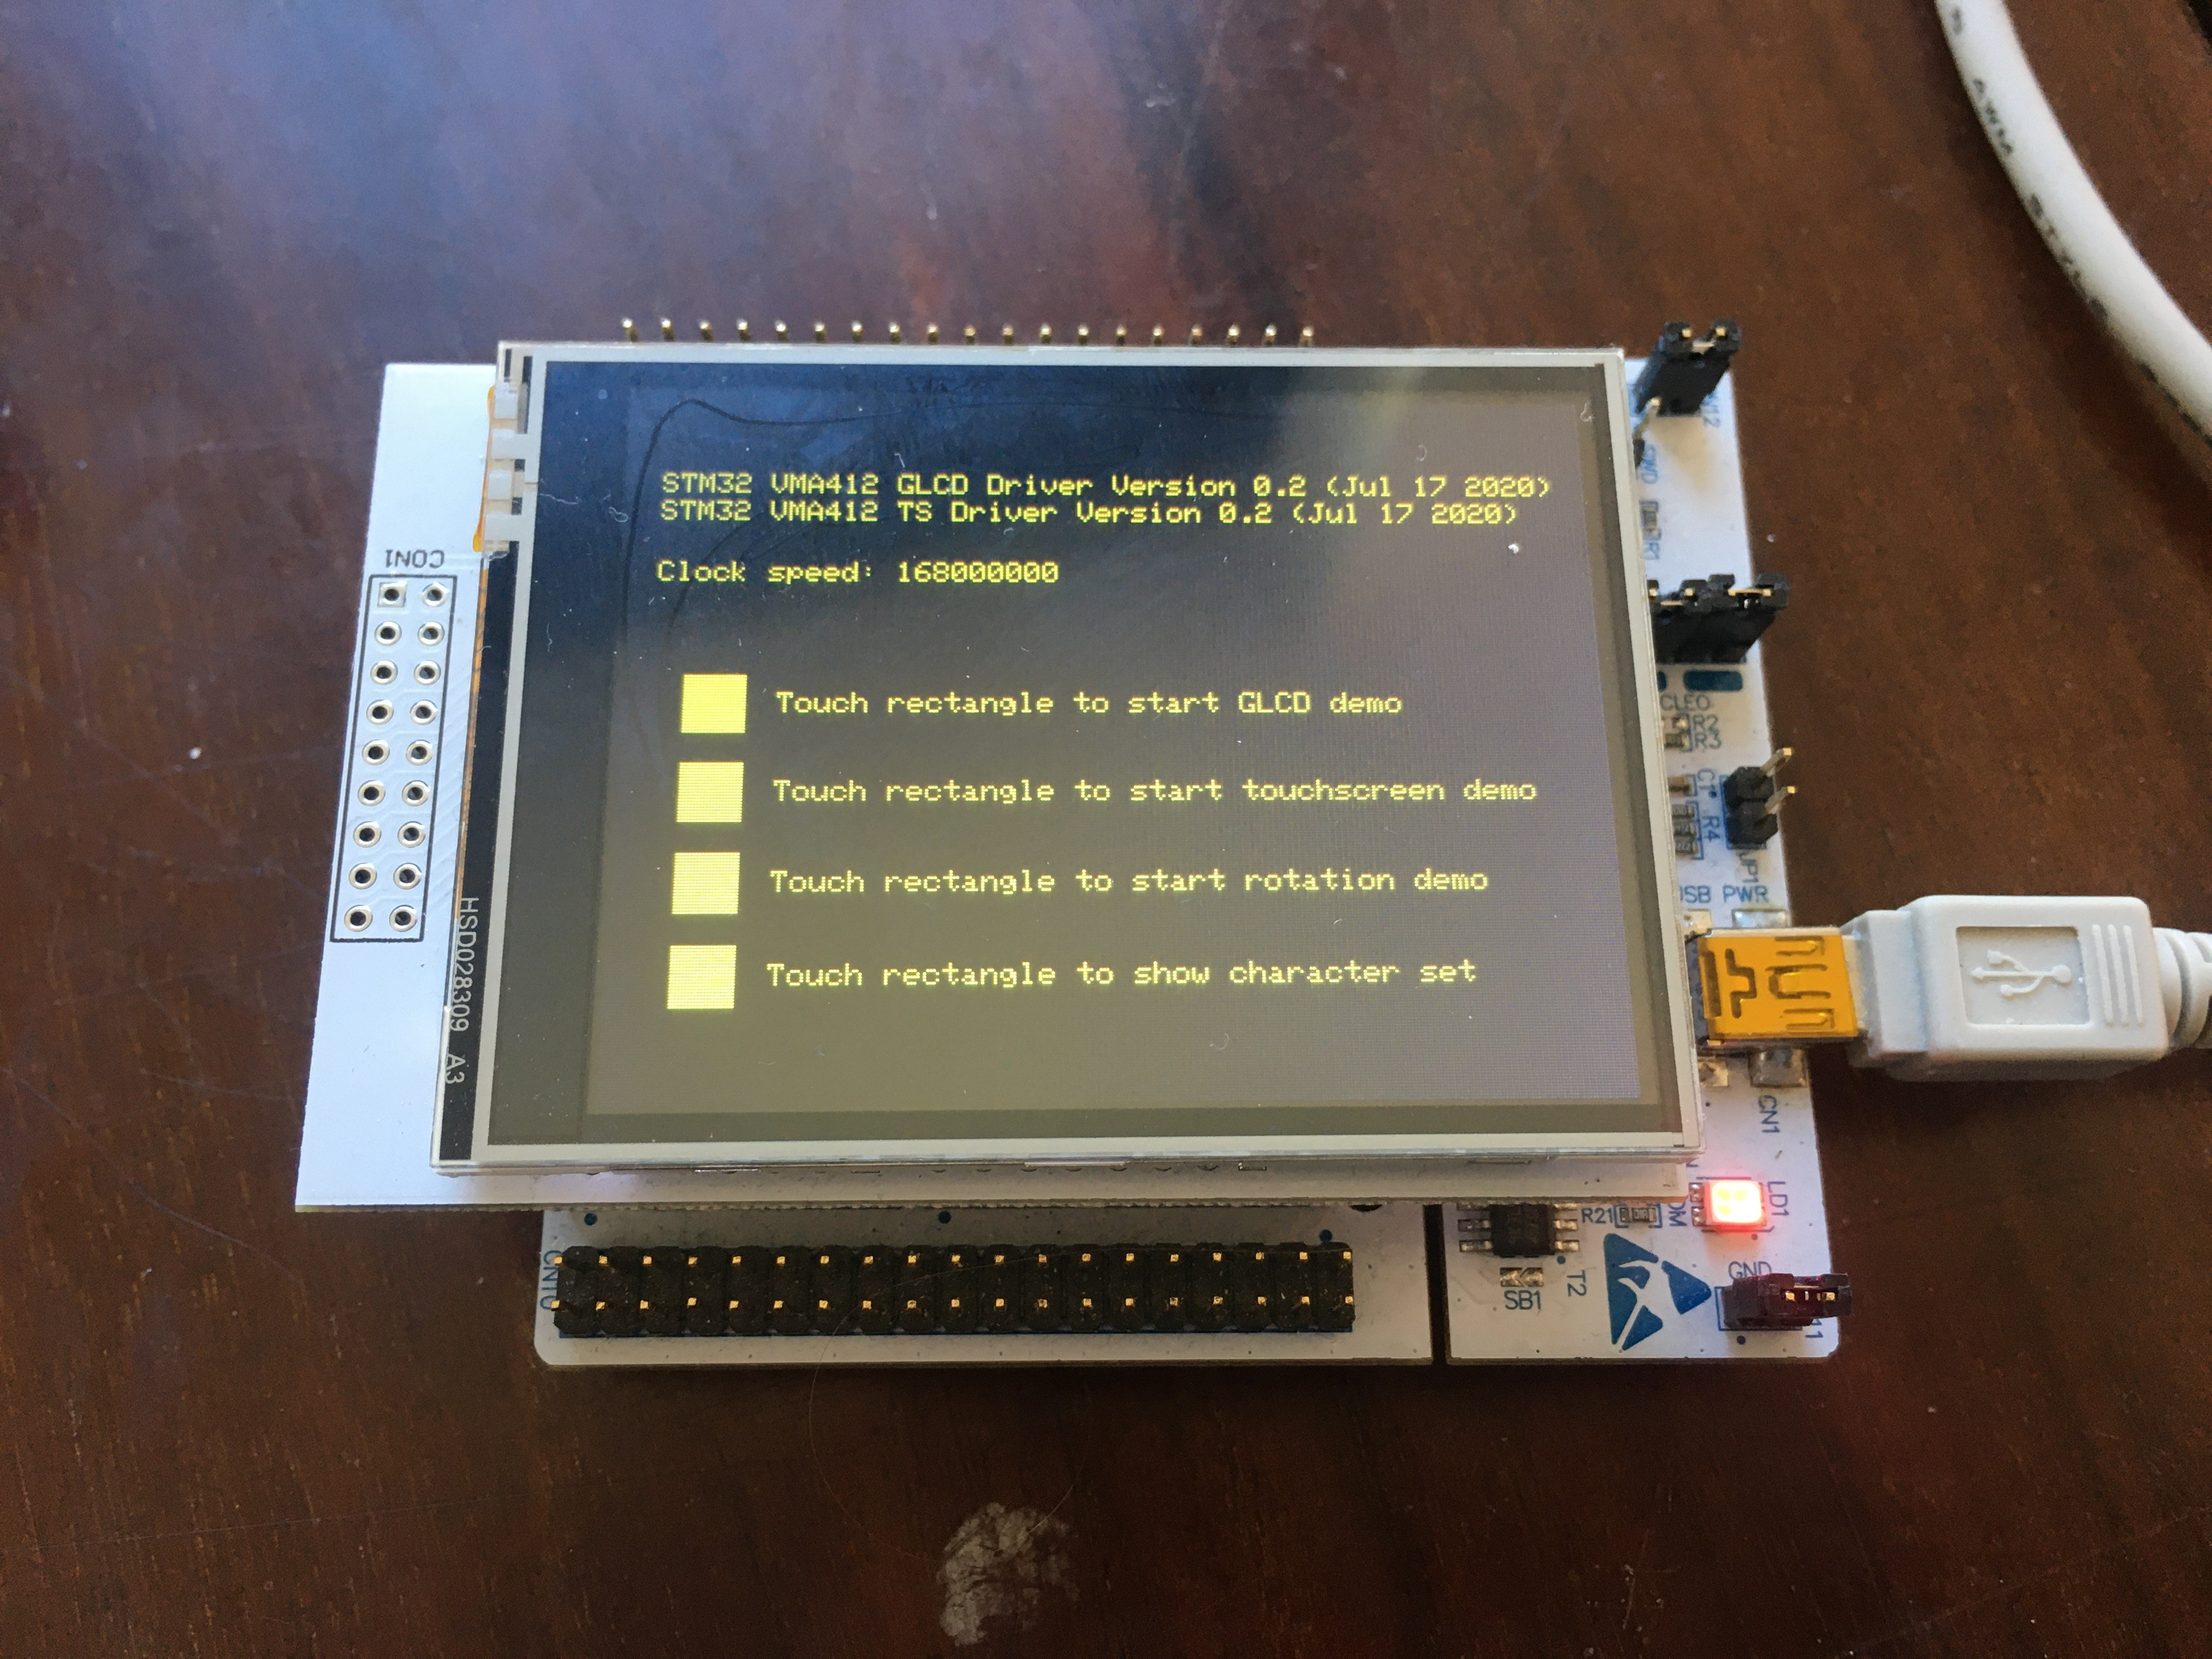
\includegraphics[width=0.7\textwidth]{start_demo}
\caption{Starting the demo.}
\label{fig:2}
\end{figure}

\begin{figure}[!ht]
\centering
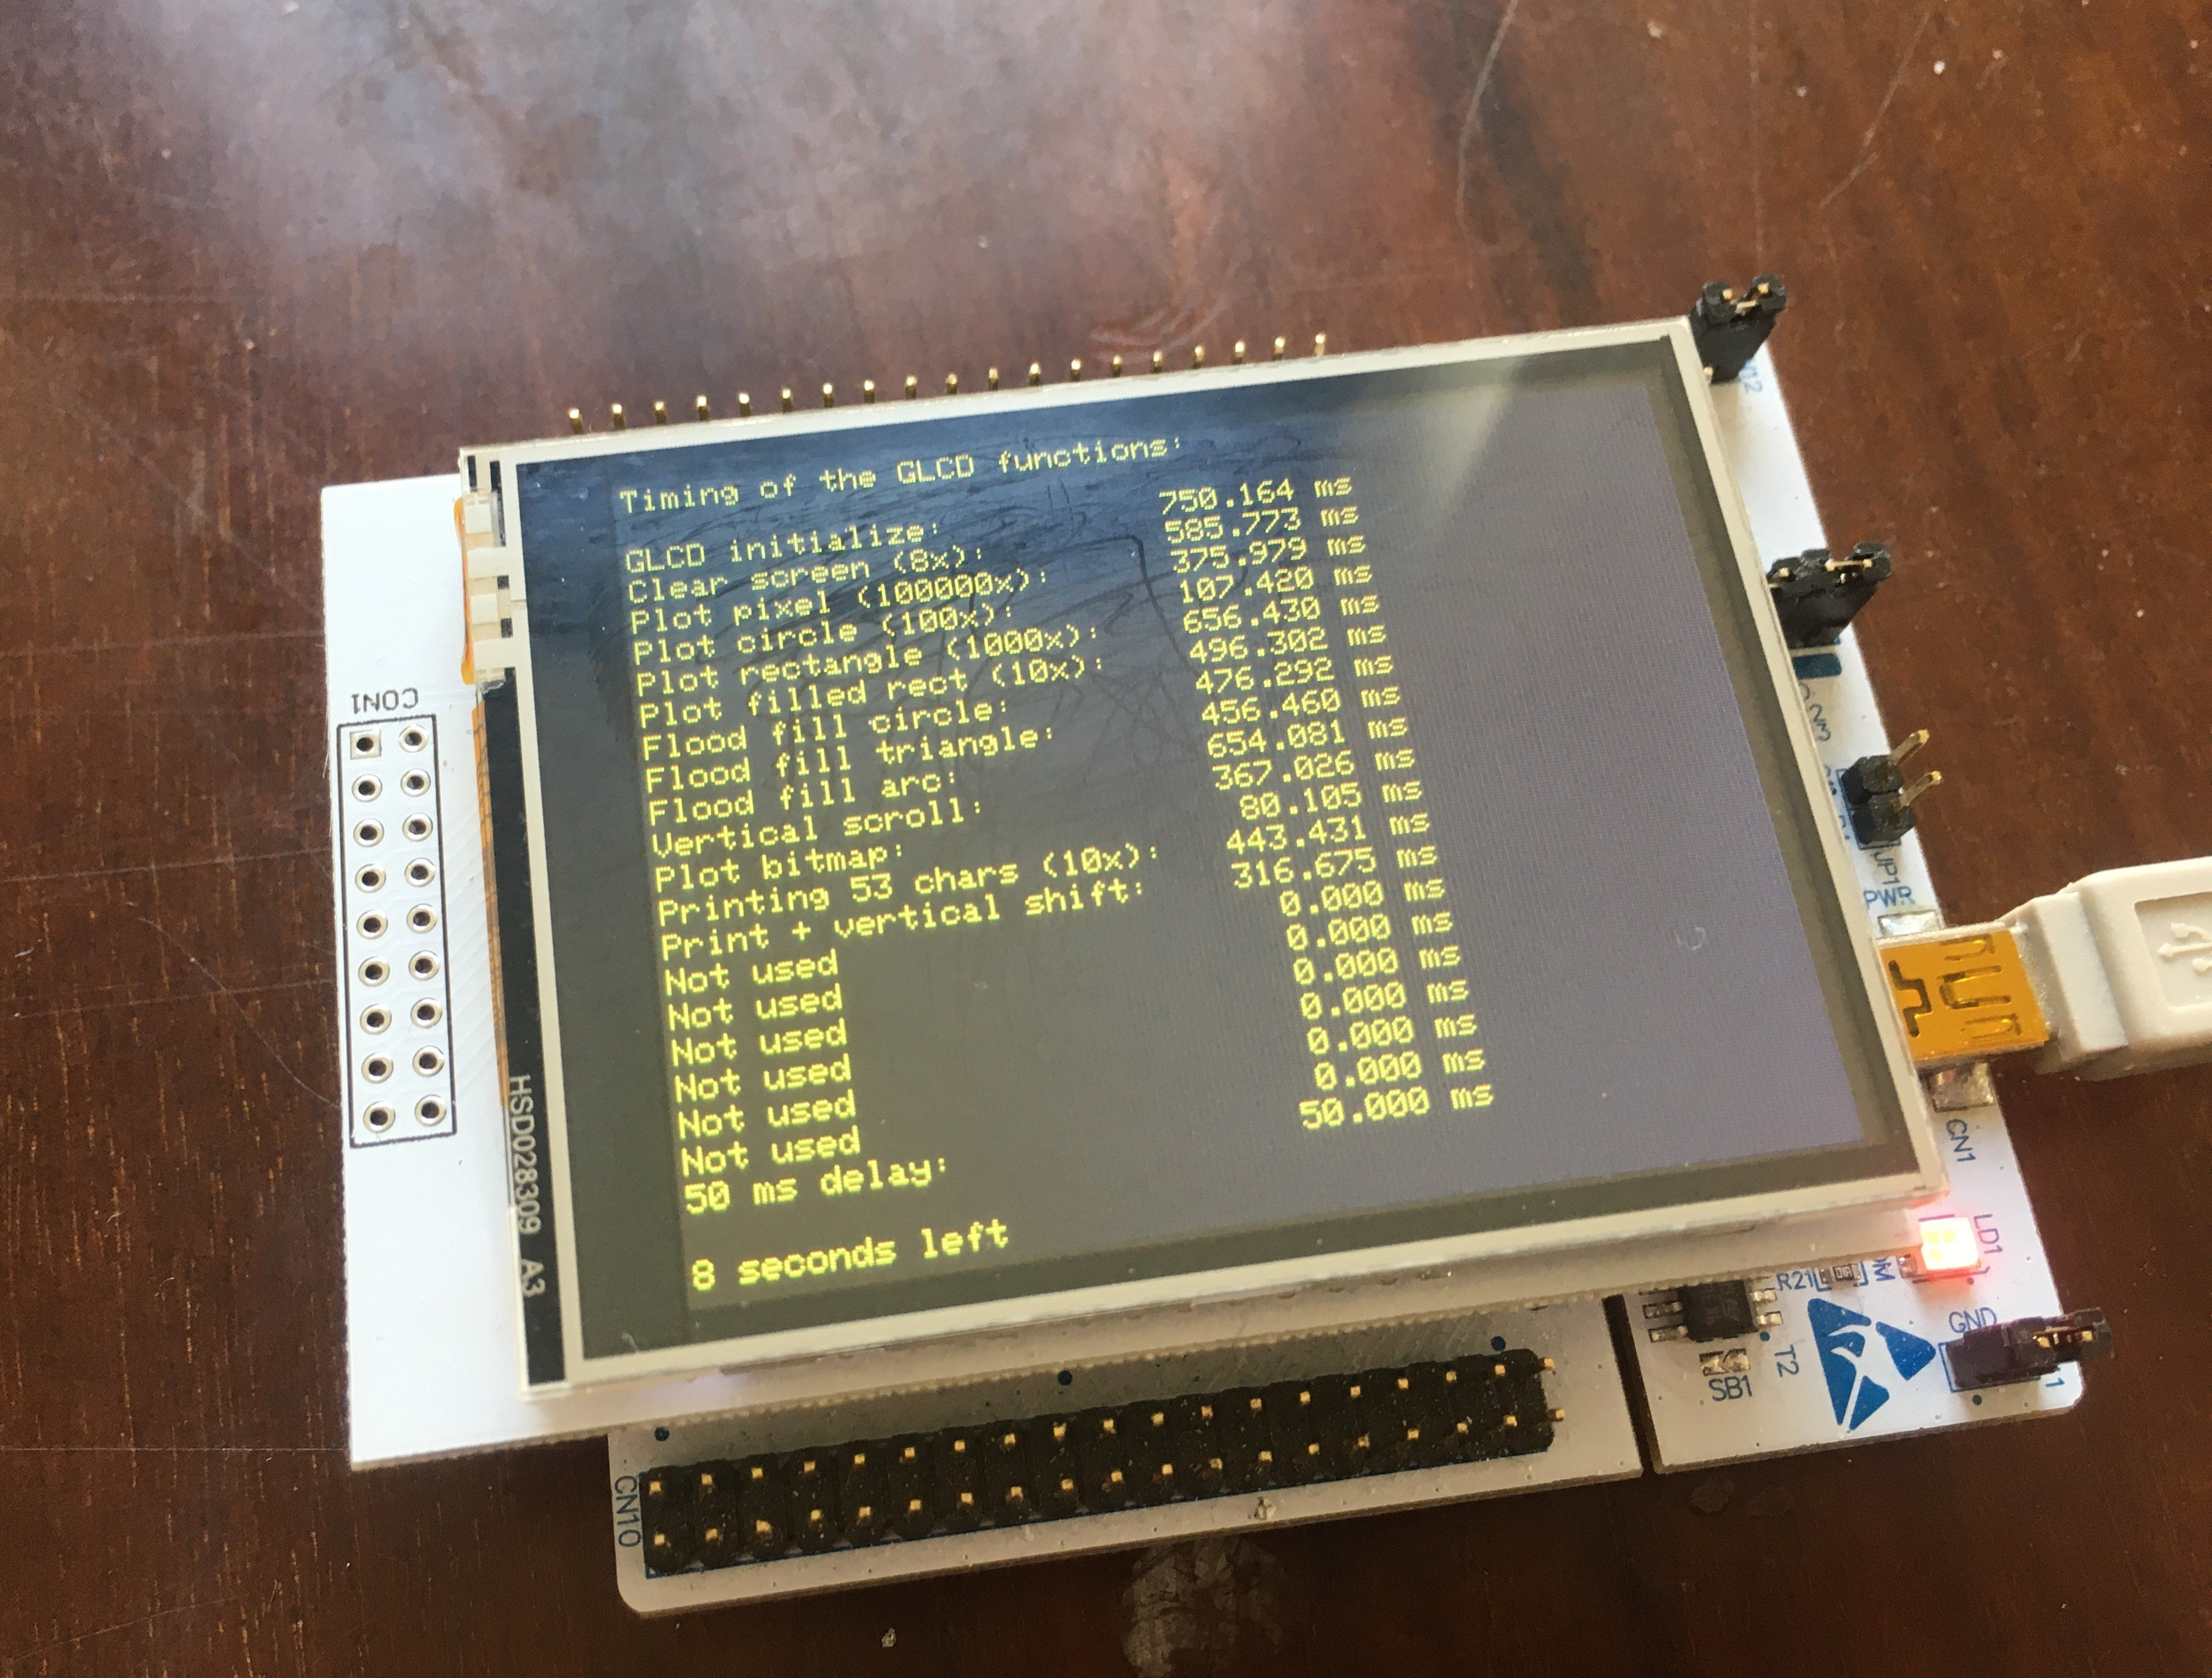
\includegraphics[width=0.7\textwidth]{times}
\caption{Displaying times for selected GLCD functions.}
\label{fig:3}
\end{figure}

\section{Color system}
The GLCD is set up to use the 18-bit color specification. This means that colors are specified with unsigned 32 bits. The specification as follows:

Bits 31-24: should be kept at 0.\\
Bits 23-16: red -- only upper 6 bits are used\\
Bits 15-8: green -- only upper 6 bits are used\\
Bits 7-0: blue -- only upper 6 bits are used

\textbf{Note:} The 16 bit color specification in \textbf{NOT} supported.

Please note that although 8 bits per color can be specified, only the upper 6 bits of each color are used, since the display uses 18 bits of color infomation. The lower 2 bits of each color are ignored.

The color is specified using the the type \lstinline|glcd_color_t|.

\subsection{Predefined colors}
There are some predefines colors:

\begin{lstlisting}
#define GLCD_COLOR_BLACK   (0x000000)
#define GLCD_COLOR_BLUE    (0x0000ff)
#define GLCD_COLOR_GREEN   (0x00ff00)
#define GLCD_COLOR_CYAN    (0x00ffff)
#define GLCD_COLOR_RED     (0xff0000)
#define GLCD_COLOR_MAGENTA (0xff00ff)
#define GLCD_COLOR_YELLOW  (0xffff00)
#define GLCD_COLOR_WHITE   (0xffffff)

#define GLCD_COLOR_GREY50  (0x7f7f7f)

/* THUAS default color */
#define GLCD_COLOR_THUASGREEN ((158<<16)|(167<<8)|0)
\end{lstlisting}

\subsection{Using your own color}
To use your own color, please use the color type \lstinline|glcd_color_t|:

\begin{lstlisting}
glcd_color_t SkyBlue2 = (126<<16)|(192<<8)|238
\end{lstlisting}

\section{X and Y coordinates}
The X and Y coordinates use type \lstinline|uint16_t| for their values. The screen is set up in landscape where \lstinline|X| is between 0 and 319 and \lstinline|y| is between 0 and 239. Point (0,0) is in the upper left corner,
point (239,319) is in the lower right corner.



\section{GLCD Initialization}
First you have to set up the clock system used by the STM32F microcontroller. If you use the onboard (but external) clock generator, make sure that the value of \lstinline|HSE_VALUE| is set to the correct frequency. In the case of the Nucleo board it is 8000000 (8 MHz). This value is defined in \lstinline|stm32f4xx_hal_conf.h| and \lstinline|system_stm32f4xx.c|.


If you use the internal HSI (\lstinline|HSIVALUE|), the frequency is 16 MHz by default. Best is to set up the clock speed to the maximum frequency allowed by the microcontroller.

Initialize the graphic VMA412 and graphic functions by calling the \lstinline|glcd_init()| function. After calling that function the display is initialized and ready for use.

\subsection{Initialize display}
This function must be called after the clock system is set up and before using any other GLCD functions. The function prototype is:
\begin{lstlisting}
void glcd_init(void);
\end{lstlisting}

Note: call this function \textbf{after} the clock system is set up.

\subsection{Setting the write delay}
\textbf{Note:} use with care.\\
Sets the delay for write actions. There is no need to call this function as the correct timing is calculated according to the system clock speed after the clock system is set up. \lstinline|delay| must be greater than 0. The function prototype is:
\begin{lstlisting}
void glcd_set_write_pulse_delay(uint32_t delay);
\end{lstlisting}


\section{GLCD low level functions}
There are a number of low level functions. They are normally not needed.

\subsection{Reading data from the display}
Te read data from the display, use the function \lstinline|glcd_read_terminate|. Reading is explictly terminated. The function prototype is:

\begin{lstlisting}
void glcd_read_terminate(uint16_t cmd,            // The command
                         uint16_t amount,         // Amount of data
                         glcd_buffer_t data[]);   // The buffer
\end{lstlisting}

\subsection{Writing data to the display}
Writes data to the display, no explicit terminate. This means that multiple writes can be done in sequence.
\begin{lstlisting}
void glcd_write(uint16_t cmd,                     // The command
                uint16_t amount,                  // Amount of data
                const glcd_buffer_t data[]);      // The buffer
\end{lstlisting}

\subsection{Explicit terminating a write}

Terminates a write:
\begin{lstlisting}
void gcld_terminate_write(void);
\end{lstlisting}

\subsection{Changing the buffer type}
The low level functions use an internal buffer. The buffer is of type \lstinline|glcd_buffer_t|. This normally set to an unsigned 16-bit size. This size can be changed:

Set to \lstinline|uint8_t| for minimal resources\\
Set to \lstinline|uint16_t| for best speed\\
Set to \lstinline|uint32_t| for maximum capacity (not recommended)
 
\section{GLCD high level commands}

\subsection{Delay}

To delay your applications (in milliseconds), use :
\begin{lstlisting}
void glcd_delay_ms(uint32_t delay);
\end{lstlisting}

\subsection{Rotating the screen}
\textbf{NOTE: rotation is currently not supported correcly.}\\

To set the rotation of the screen, use:
\begin{lstlisting}
void glcd_setrotation(glcd_rotation_t rot);
\end{lstlisting}

Where \lstinline|rot| is one of:

\begin{lstlisting}
GLCD_SCREEN_ROT0           // Standard landscape, default
GLCD_SCREEN_ROT90          // Rotate 90 degrees
GLCD_SCREEN_ROT180         // Rotate 180 degrees
GLCD_SCREEN_ROT270         // Rotate 270 degrees
\end{lstlisting}

\subsection{Clear the screen}
To clear the screen with a color, use:
\begin{lstlisting}
void glcd_cls(glcd_color_t color);
\end{lstlisting}

\subsection{Plot a pixel}
To plot a pixel, use:
\begin{lstlisting}
void glcd_plotpixel(uint16_t x,           // x coordinate
                    uint16_t y,           // y coordinate
                    glcd_color_t color);  // color
\end{lstlisting}

\subsection{Read a pixel}
To read a pixel (getting color information), use:

\begin{lstlisting}
glcd_color_t glcd_readpixel(uint16_t x,   // x coordinate
                            uint16_t y);  // y coordinate
\end{lstlisting}

\subsection{Plot a horizontal line}
To plot a horizontal line (fast), use:
\begin{lstlisting}
void glcd_plothorizontalline(uint16_t x,           // x coordinate
                             uint16_t y,           // y coordinate
                             uint16_t w,           // width
                             glcd_color_t color);  // color
\end{lstlisting}


\subsection{Plot a vertical line}
To plot a vertical line (fast), use:
\begin{lstlisting}
void glcd_plotverticalline(uint16_t x              // x coordinate
                           uint16_t y,             // y coordinate
                           uint16_t h,             // height
                           glcd_color_t color);    // color
\end{lstlisting}

\subsection{Plot a line with any angle and length}
To plot a line with any angle and length, use:
\begin{lstlisting}
void glcd_plotline(uint16_t x0,            // x start point
                   uint16_t y0,            // y start point
                   uint16_t x1,            // z end point
                   uint16_t y1,            // y end point
                   glcd_color_t color);    // color
\end{lstlisting}

\subsection{Plot a character using buildin font}
To plot a character using the buildin fond (5x8), use:
\begin{lstlisting}
void glcd_plotchar(uint16_t x,             // x coordinate
                   uint16_t y,             // y coordinate
                   uint8_t c,              // character (0-255)
                   glcd_color_t color,     // color
                   glcd_color_t bg);       // background color
\end{lstlisting}

Note: character is one of 0 -- 255 (no special C treatment)\\
Note: if \lstinline|color| is equal to \lstinline|bg| then pixels having background color are not printed! 

\subsection{Plot a string using buildin font}
To plot a string using the buildin font, use:
\begin{lstlisting}
void glcd_plotstring(uint16_t x,                  // x coordinate
                     uint16_t y,                  // y coordinate
                     char str[],                  // the string
                     glcd_color_t color,          // color
                     glcd_color_t bg,             // background color
                     glcd_spacing_t spacing);     // spacing
\end{lstlisting}

Note: a \lstinline|\0| terminates a string (as in C)\\
Note: if \lstinline|color| is equal to \lstinline|bg| then pixels having background color are not printed! 
Note: \lstinline|spacing| is one of:
\begin{lstlisting}
GLCD_STRING_CONDENSED  // zero pixels apart
GLCD_STRING_NORMAL     // one pixel apart
GLCD_STRING_WIDE       // two pixels apart
\end{lstlisting}

\subsection{Plot a rectangle}
To plot a rectangle, use:
\begin{lstlisting}
void glcd_plotrect(uint16_t x,             // x coordinate
                   uint16_t y,             // y coordinate
                   uint16_t w,             // width
                   uint16_t h,             // height
                   glcd_color_t color);    // color
\end{lstlisting}

\subsection{Plot a filled recangle}
To plot a filled rectangle, use:
\begin{lstlisting}
void glcd_plotrectfill(uint16_t x,            // x coordinate
                       uint16_t y,            // y coordinate
                       uint16_t w,            // width
                       uint16_t h,            // height
                       glcd_color_t color);   // color
\end{lstlisting}

\subsection{Plot a circle}
To plot a circle, use:
\begin{lstlisting}
void glcd_plotcircle(uint16_t x0,             // center x coordinate
                     uint16_t y0,             // center y coordinate
                     uint16_t r,              // radius
                     glcd_color_t color);     // color
\end{lstlisting}

\subsection{Plot an arc}
To plot an arc, use:
\begin{lstlisting}
void glcd_plotarc(uint16_t xc,                // center x coordinate
                  uint16_t yc,                // center y coordinate
                  uint16_t r,                 // radius
                  float start,                // start angle in degrees
                  float stop,                 // stop angle in degrees
                  glcd_color_t color);        // color
\end{lstlisting}

Note: this function is only available if \lstinline|GLCD_USE_ARC| is defined.\\
Note: this function uses \lstinline|sinf| and \lstinline|cosf| math functions, using the onboard FPU.

\subsection{Plot a 2-color bitmap}
To plot a 2-color bitmap, use:
\begin{lstlisting}
void glcd_plotbitmap(uint16_t x,              // x coordinate
                     uint16_t y,              // y coordinate
                     const uint8_t bitmap[],  // the bitmap, see note
                     uint16_t w,              // width
                     uint16_t h,              // height
                     glcd_color_t color,      // color
                     glcd_color_t bg);        // background color
\end{lstlisting}

Note: \lstinline|bitmap| consists of bytes (\lstinline|uint8_t|). A 1 in a byte is converted to \lstinline|color|, a 0 in a byte is converted to \lstinline|bg|.

\subsection{Display inversion}
Sets the display inversion (or not):
\begin{lstlisting}
void glcd_inversion(glcd_display_inversion_t what);
\end{lstlisting}

Note: \lstinline|what| is one of:
\begin{lstlisting}
GLCD_DISPLAY_INVERSION_OFF
GLCD_DISPLAY_INVERSION_ON
\end{lstlisting}

\subsection{Display idle}
Set the display to idle (or not):
\begin{lstlisting}
void glcd_idle(glcd_display_idle_t what);
\end{lstlisting}

Note: \lstinline|what| is one of:

\begin{lstlisting}
GLCD_DISPLAY_IDLE_OFF
GLCD_DISPLAY_IDLE_ON
\end{lstlisting}

\subsection{Display ON or OFF}
Sets the display on or off:
\begin{lstlisting}
void glcd_display(glcd_display_t what);
\end{lstlisting}

Note: \lstinline|what| is one of

\begin{lstlisting}
GLCD_DISPLAY_OFF
GLCD_DISPLAY_ON
\end{lstlisting}

\subsection{Flood fill an object}
Flood fill an object using a stack based approach:
\begin{lstlisting}
void glcd_floodfill(uint16_t xs,                 // x start point
                    uint16_t ys,                 // y start point
                    glcd_color_t fillColor,      // color for pixel == 1
                    glcd_color_t defaultColor);  // color for pixel == 0
\end{lstlisting}

Note: this function is only available if \lstinline|GLCD_USE_FLOOD_FILL| is defined.\\
Note: set \lstinline|GLCD_STACK_SIZE| to an appropiate value.\\
Note: if you have problems filling an object increase the value of \lstinline|GLCD_STACK_SIZE|.\\
Note: the stack uses unsigned 32-bit entries so the complete stack uses \lstinline|GLCD_STACK_SIZE|*4 bytes of RAM.

\subsection{Scroll the display vertical upwards}
To scroll the display vertical a number of lines, use:
\begin{lstlisting}
void glcd_scrollvertical(uint16_t lines);   // lines to scroll upwards
\end{lstlisting}

Note: this is a software based scroll, could be slow. The lines are scrolled upwards off the screen (no rotation), and the vacant lines are left untouched.

\subsection{Console based character printing}
\label{sec:consolebasedcharacterprinting}
To use a simple console based character printing, use:
\begin{lstlisting}
void glcd_putchar(char c);
\end{lstlisting}

Note: characters are printed in yellow, background is black\\
Note: \lstinline|\f| (form feed) clears the screen\\
Note: \lstinline|\n| returns and goes to the next line\\
Note: \lstinline|\r| return to the beginning of the line\\
Note: \lstinline|\b| erases last character and goes one character back (ultimate to the beginning of the line)\\
Note: all other characters are printed using the internal font\\
Note: if a character ``falls off'' the display, line wrap will be used, may cause a vertical shift\\
Note: \lstinline|\t| is currenty not handled
\subsection{Console based string printing}
To use a simple console based string printing use:
\begin{lstlisting}
void glcd_printconsole(char str[]);
\end{lstlisting}

Note: see $\S$\ref{sec:consolebasedcharacterprinting} for character handling.

\subsection{Get the current screen width}
To get the current screen width, use:

\begin{lstlisting}
uint16_t glcd_getwidth(void);
\end{lstlisting}

\subsection{Get the current screen height}
To get the current screen height, use:
\begin{lstlisting}
uint16_t glcd_getheight(void);
\end{lstlisting}




\section{GLCD Tayloring}
There are a number of \lstinline|#define|'s that can be manipulated to taylor the GLCD functions to your needs. They can be found in \lstinline|glcd_ili9341_vma412.h|:

\begin{lstlisting}
#define GLCD_USE_FLOOD_FILL
#define GLCD_STACK_SIZE (2000)
#define GLCD_USE_FLOOD_FILL_PRINT_IF_STACK_OVERFLOW
#define GLCD_USE_ARC

#define GLCD_WIDTH (320)
#define GLCD_HEIGHT (240)
\end{lstlisting}

Define \lstinline|GLCD_USE_FLOOD_FILL| if you need to (flood) fill objects, undefine to save ROM  and RAM resources. If you use flood fill, set the stack size \lstinline|GLCD_STACK_SIZE| to an appropriate size. While testing or debugging, define \lstinline|GLCD_USE_FLOOD_FILL_PRINT_IF_STACK_OVERFLOW|. This will print warning messages if there is a stack overflow when filling objects. Undefine if you are sure there will be no stack overflow. Define \lstinline|GLCD_USE_ARC| if you need to plot arcs, undefine to save ROM resources. Plotting arcs use the onboard FPU for sine and cosine calculations.

Leave \lstinline|GLCD_WIDTH| and \lstinline|GLCD_HEIGHT| to their respective values.

The GLCD functions use an internal buffer. The size of the buffer elements are set to the type \lstinline|glcd_buffer_t|. This is normally set to unsigned 16-bit. The buffer length is set to \lstinline|GLCD_WIDTH|*3+1.

The size of the buffer elements can be changed:

\begin{lstlisting}
typedef uint16_t glcd_buffer_t;
\end{lstlisting}

Set to \lstinline|uint8_t| for smallest RAM footprint. Set to \lstinline|uint16_t| for fastest processing. There is no speed gain when setting to \lstinline|uint32_t|. It just wastes resources.

\section{Touchscreen Initialization}
Before using any of the touchscreen functions, you have to initialize the touchscreen. Reading the X and Y coordinates of the pressed screen points needs one of the onboard ADC's. The function \lstinline|touchscreen_init| initializes the selected ADC. Please note that the selected ADC must be dedicated to the touchscreen functions, since the ADC is setup only once. Sharing the ADC with other functions is not recommended.

Please note that the ADC is setup for 10-bit conversions so the values returned are from 0 to 1023 (inclusive).

\section{Touchscreen low level functions}
There are none.

\section{Touchscreen high level functions}

\subsection{Initializing the touchscreen}
To initialize the touchscreen, use:

\begin{lstlisting}
uint32_t touchscreen_init(ADC_TypeDef *used_ADC);
\end{lstlisting}

Note: this function must be called after the clock system is set up.\\
Note: \lstinline|used_ADC| is an ADC handle. Currently only \lstinline|ADC1| and \lstinline|ADC2| are supported. \lstinline|ADC3| is currently \textbf{not} supported.\\
Note: if the initialization succeeds an 1 is return, if failing a 0 is returned.

\subsection{Read raw X position}
To read the current raw X position, use:

\begin{lstlisting}
uint32_t touchscreen_readx(void);
\end{lstlisting}

Note: this value is only of interest if the touchscreen is pressed\\
Note: returns the raw X position from the screen. This value is an indication of where the screen is pressed. It is not the actual X position as can be used with the GLCD functions. You need to map the raw X position.

\subsection{Read raw Y position}
To read the current raw y position, use:

\begin{lstlisting}
uint32_t touchscreen_ready(void);
\end{lstlisting}

Note: this value is only of interest if the touchscreen is pressed\\Note: returns the raw Y position from the screen. This value is an indication of where the screen is pressed. It is not the actual Y position as can be used with the GLCD functions. You need to map the raw Y position.

\subsection{Read raw pressure}
To read the raw pressure, use:

\begin{lstlisting}
uint32_t touchscreen_pressure(void);
\end{lstlisting}

Note: if the touch screen is \textbf{not} pressed this functions returns a small number, typically 0. Any other values means that the touchscreen is pressed.

\subsection{Mapping the raw X and Y values to screen coordinates}
To map raw X and Y values to screen coordinates, use:

\begin{lstlisting}
int32_t touchscreen_map(uint32_t value,
                        uint32_t tlow,
                        uint32_t thigh,
                        uint32_t slow,
                        uint32_t shigh);
\end{lstlisting}

Note: \lstinline|value| is the raw value from X or Y\\
Note: \lstinline|tlow| is lowest raw touchscreen value (X and Y)\\
Note: \lstinline|thigh| is highest raw touchscreen value (X and Y)\\
Note: \lstinline|slow| is lowest GLCD screen value (X and Y)\\
Note: \lstinline|shigh| is highest GLCD screen value (X and Y)\\
Note: \lstinline|thigh| must be greater than \lstinline|tlow|

Note: the returned value can be negative. This is an indication that the touchscreen is not calibrated correctly.\\
Note: this function internally uses floats to do the calculations. This will be done using the onboard FPU.

The map function corresponds to the linear equation:

\begin{equation}
returned\ value = a\cdot value + b
\end{equation}

where $a$ is

\begin{equation}
a = \frac{shigh-slow}{thigh-tlow}\qquad\qquad(thigh>tlow)
\end{equation}

and $b$ is

\begin{equation}
b = - a\cdot tlow;
\end{equation}

Note: if $thigh \leq tlow$ the value 0 is returned.

\subsection{Testing if the touchscreen is pressed}
To test whether the screen is touched, use:

\begin{lstlisting}
uint32_t touchscreen_pressed(uint32_t p);
\end{lstlisting}

Note: \lstinline|p| is the raw pressure value

Note: a 1 is returned is touchscreen is pressed\\
Note: a 0 is returned is touchscreen is not pressed\\

\section{Calibrating the touchscreen}
The touchscreen of the Velleman VMA412 is constructed of resistive foils. Normally the resistance and hence the voltage measured is linear propotional to the location where the touchscreen is pressed. Small deficienties during fabrication produce differences between samples of the screens. To compensatie for that, calibration is needed. There are a number of \lstinline|#define|'s to calibrate the screen. These can be found in \lstinline|touchscreen_vma412.h|.

The outer left raw position is set with \lstinline|TOUCH_LEFT|. The outer right raw position is set with \lstinline|TOUCH_RIGHT|. The outer top raw position is set with \lstinline|TOUCH_TOP|. The outer bottom raw position is set with \lstinline|TOUCH_BOTTOM|.

Whether the touchscreen is pressed or not is calculated according to raw touchscreen values. The lower bound for pressed is set with \lstinline|TOUCH_PRESSURE_LOW|. The upper bound for pressed is set with \lstinline|TOUCH_PRESSURE_HIGH|.

Note all values must be within the values 0 to 1023 (inclusive).

Reading raw values is done by oversamping and then the mean of the samples is returned. You can set the number of oversamples using the define \lstinline|TOUCH_SAMPLES|. The default value is 16. This value must be 2 or greater.

\section{Debugging or production use}
If you need to debug the functions, set the compiler optimization to \lstinline|-O0| (no optimization) or \lstinline|-Og| (optimize for debug). If you want to exhibit full speed support set the optimization to \lstinline|-Ofast|. If you need the smallest ROM footprint and have some speed, set the optimization to \lstinline|-Os|.

\section{Nice tricks}
To wait until the touchscreen is touched, use one of

\begin{lstlisting}
while (p = touchscreen_pressure(), !touchscreen_pressed(p)) {}
while (!touchscreen_pressed(touchscreen_pressure())) {}
\end{lstlisting}




\section{Todo's}
Some todo's left:

\begin{itemize}
\item Quarter circle plot function, with fill option, will be faster than flood fill circles;
\item Triangle plot function;
\item Regular polygon plot function;
\item Exchange top/bottom and left/right;
\item Fix printing for rotation 180 and 270;
\item More testing on rotated screen/touchscreens
\item Handling of \lstinline|\t| in console based printing
\end{itemize}


\end{document}
